\documentclass{standalone}
\usepackage{tikz}
\usetikzlibrary{patterns, positioning}

\begin{document}
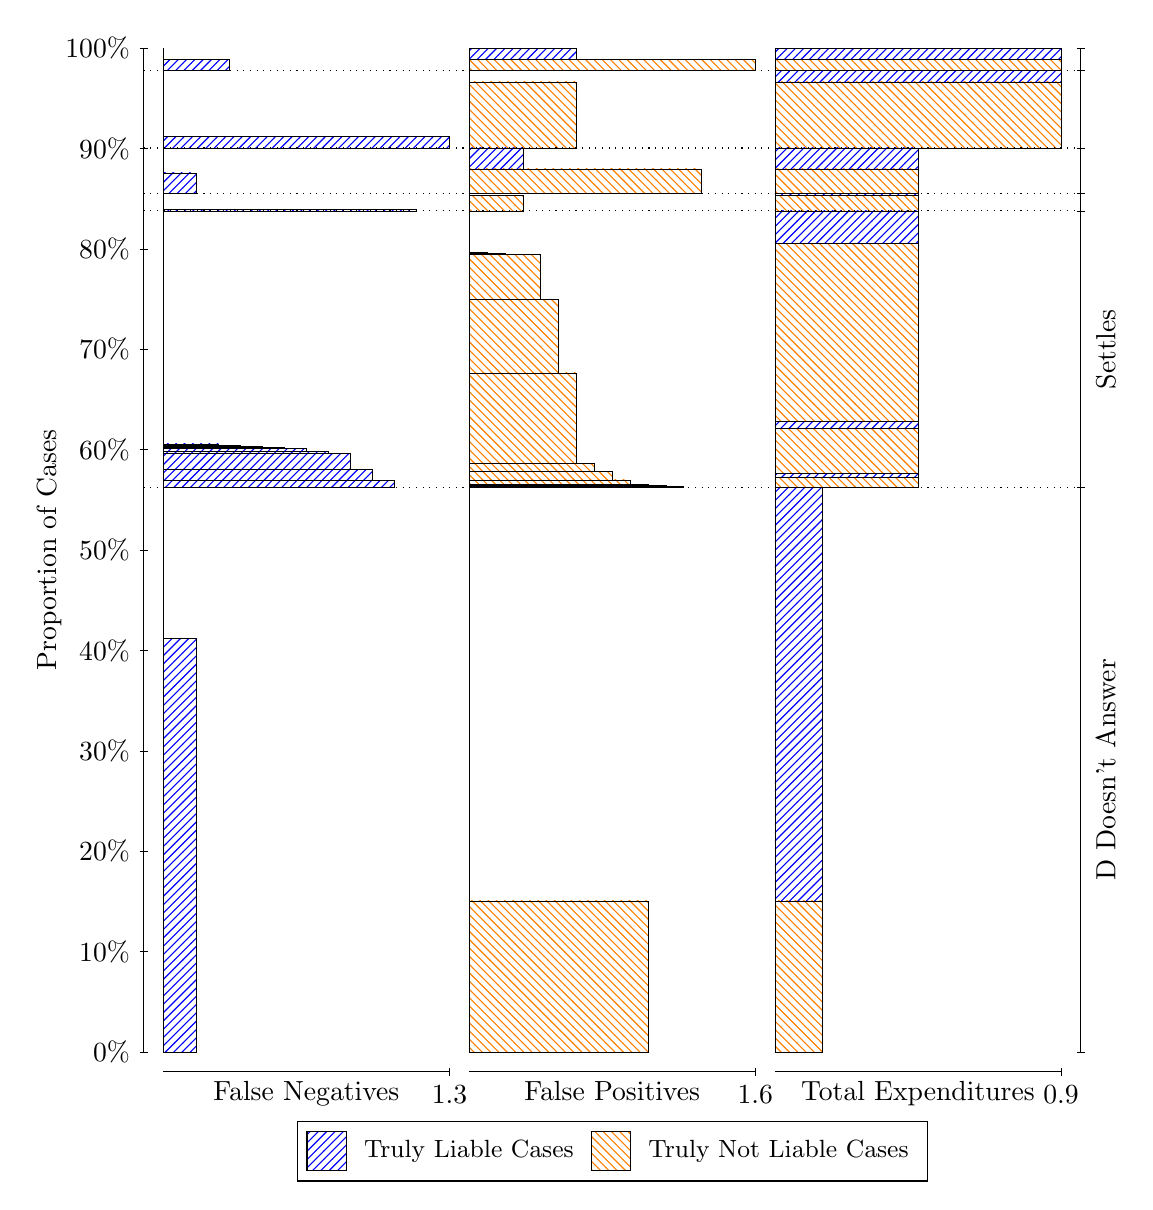
\begin{tikzpicture}
\draw[black, very thin] (1.5,1.75) -- (1.5,14.5);
\node[rotate=90, anchor=center] at (0.3, 8.125) {Proportion of Cases};
\draw[black, very thin] (1.45,1.75) -- (1.55,1.75);
\node[anchor=east] at (1.45, 1.75) {0\%};
\draw[black, very thin] (1.45,3.025) -- (1.55,3.025);
\node[anchor=east] at (1.45, 3.025) {10\%};
\draw[black, very thin] (1.45,4.3) -- (1.55,4.3);
\node[anchor=east] at (1.45, 4.3) {20\%};
\draw[black, very thin] (1.45,5.575) -- (1.55,5.575);
\node[anchor=east] at (1.45, 5.575) {30\%};
\draw[black, very thin] (1.45,6.85) -- (1.55,6.85);
\node[anchor=east] at (1.45, 6.85) {40\%};
\draw[black, very thin] (1.45,8.125) -- (1.55,8.125);
\node[anchor=east] at (1.45, 8.125) {50\%};
\draw[black, very thin] (1.45,9.4) -- (1.55,9.4);
\node[anchor=east] at (1.45, 9.4) {60\%};
\draw[black, very thin] (1.45,10.675) -- (1.55,10.675);
\node[anchor=east] at (1.45, 10.675) {70\%};
\draw[black, very thin] (1.45,11.95) -- (1.55,11.95);
\node[anchor=east] at (1.45, 11.95) {80\%};
\draw[black, very thin] (1.45,13.225) -- (1.55,13.225);
\node[anchor=east] at (1.45, 13.225) {90\%};
\draw[black, very thin] (1.45,14.5) -- (1.55,14.5);
\node[anchor=east] at (1.45, 14.5) {100\%};

\draw[black, very thin] (13.4,1.75) -- (13.4,14.5);
\draw[black, very thin] (13.35,1.75) -- (13.45,1.75);
\node[anchor=west] at (13.35, 1.75) {};
\draw[black, very thin] (13.35,8.9176) -- (13.45,8.9176);
\node[anchor=west] at (13.35, 8.9176) {};
\draw[black, very thin] (13.35,12.431) -- (13.45,12.431);
\node[anchor=west] at (13.35, 12.431) {};
\draw[black, very thin] (13.35,12.65) -- (13.45,12.65);
\node[anchor=west] at (13.35, 12.65) {};
\draw[black, very thin] (13.35,13.231) -- (13.45,13.231);
\node[anchor=west] at (13.35, 13.231) {};
\draw[black, very thin] (13.35,14.215) -- (13.45,14.215);
\node[anchor=west] at (13.35, 14.215) {};
\draw[black, very thin] (13.35,14.5) -- (13.45,14.5);
\node[anchor=west] at (13.35, 14.5) {};

\draw[black, very thin, pattern color=blue, pattern=north east lines] (1.75,1.75) rectangle (2.1692,6.9994);
\draw[black, very thin, pattern color=orange, pattern=north west lines] (1.75,6.9994) rectangle (1.75,8.9176);
\draw[black, very thin, pattern color=blue, pattern=north east lines] (1.75,8.9176) rectangle (4.6846,9.0063);
\draw[black, very thin, pattern color=blue, pattern=north east lines] (1.75,9.0063) rectangle (4.4051,9.1512);
\draw[black, very thin, pattern color=blue, pattern=north east lines] (1.75,9.1512) rectangle (4.1256,9.3509);
\draw[black, very thin, pattern color=blue, pattern=north east lines] (1.75,9.3509) rectangle (3.8462,9.3815);
\draw[black, very thin, pattern color=blue, pattern=north east lines] (1.75,9.3815) rectangle (3.5667,9.4135);
\draw[black, very thin, pattern color=blue, pattern=north east lines] (1.75,9.4135) rectangle (3.2872,9.4316);
\draw[black, very thin, pattern color=blue, pattern=north east lines] (1.75,9.4316) rectangle (3.0077,9.444);
\draw[black, very thin, pattern color=blue, pattern=north east lines] (1.75,9.444) rectangle (2.7282,9.4523);
\draw[black, very thin, pattern color=blue, pattern=north east lines] (1.75,9.4523) rectangle (2.4487,9.4732);
\draw[black, very thin, pattern color=orange, pattern=north west lines] (1.75,9.4732) rectangle (1.75,12.431);
\draw[black, very thin, pattern color=blue, pattern=north east lines] (1.75,12.431) rectangle (4.9641,12.448);
\draw[black, very thin, pattern color=orange, pattern=north west lines] (1.75,12.448) rectangle (1.75,12.65);
\draw[black, very thin, pattern color=blue, pattern=north east lines] (1.75,12.65) rectangle (2.1692,12.915);
\draw[black, very thin, pattern color=orange, pattern=north west lines] (1.75,12.915) rectangle (1.75,13.231);
\draw[black, very thin, pattern color=blue, pattern=north east lines] (1.75,13.231) rectangle (5.3833,13.375);
\draw[black, very thin, pattern color=orange, pattern=north west lines] (1.75,13.375) rectangle (1.75,14.215);
\draw[black, very thin, pattern color=blue, pattern=north east lines] (1.75,14.215) rectangle (2.5885,14.359);
\draw[black, very thin, pattern color=orange, pattern=north west lines] (1.75,14.359) rectangle (1.75,14.5);
\draw[black, very thin, pattern color=orange, pattern=north west lines] (5.6333,1.75) rectangle (7.9042,3.6681);
\draw[black, very thin, pattern color=blue, pattern=north east lines] (5.6333,3.6681) rectangle (5.6333,8.9176);
\draw[black, very thin, pattern color=orange, pattern=north west lines] (5.6333,8.9176) rectangle (8.3583,8.9318);
\draw[black, very thin, pattern color=orange, pattern=north west lines] (5.6333,8.9318) rectangle (8.1313,8.9416);
\draw[black, very thin, pattern color=orange, pattern=north west lines] (5.6333,8.9416) rectangle (7.9042,8.9579);
\draw[black, very thin, pattern color=orange, pattern=north west lines] (5.6333,8.9579) rectangle (7.6771,9.0157);
\draw[black, very thin, pattern color=orange, pattern=north west lines] (5.6333,9.0157) rectangle (7.45,9.1204);
\draw[black, very thin, pattern color=orange, pattern=north west lines] (5.6333,9.1204) rectangle (7.2229,9.2223);
\draw[black, very thin, pattern color=orange, pattern=north west lines] (5.6333,9.2223) rectangle (6.9958,10.374);
\draw[black, very thin, pattern color=orange, pattern=north west lines] (5.6333,10.374) rectangle (6.7687,11.309);
\draw[black, very thin, pattern color=orange, pattern=north west lines] (5.6333,11.309) rectangle (6.5417,11.875);
\draw[black, very thin, pattern color=blue, pattern=north east lines] (5.6333,11.875) rectangle (6.0875,11.896);
\draw[black, very thin, pattern color=blue, pattern=north east lines] (5.6333,11.896) rectangle (5.8604,11.905);
\draw[black, very thin, pattern color=blue, pattern=north east lines] (5.6333,11.905) rectangle (5.6333,12.431);
\draw[black, very thin, pattern color=orange, pattern=north west lines] (5.6333,12.431) rectangle (6.3146,12.633);
\draw[black, very thin, pattern color=blue, pattern=north east lines] (5.6333,12.633) rectangle (5.6333,12.65);
\draw[black, very thin, pattern color=orange, pattern=north west lines] (5.6333,12.65) rectangle (8.5854,12.966);
\draw[black, very thin, pattern color=blue, pattern=north east lines] (5.6333,12.966) rectangle (6.3146,13.231);
\draw[black, very thin, pattern color=orange, pattern=north west lines] (5.6333,13.231) rectangle (6.9958,14.071);
\draw[black, very thin, pattern color=blue, pattern=north east lines] (5.6333,14.071) rectangle (5.6333,14.215);
\draw[black, very thin, pattern color=orange, pattern=north west lines] (5.6333,14.215) rectangle (9.2667,14.355);
\draw[black, very thin, pattern color=blue, pattern=north east lines] (5.6333,14.355) rectangle (6.9958,14.5);
\draw[black, very thin, pattern color=orange, pattern=north west lines] (9.5167,1.75) rectangle (10.122,3.6681);
\draw[black, very thin, pattern color=blue, pattern=north east lines] (9.5167,3.6681) rectangle (10.122,8.9176);
\draw[black, very thin, pattern color=orange, pattern=north west lines] (9.5167,8.9176) rectangle (11.333,9.0484);
\draw[black, very thin, pattern color=blue, pattern=north east lines] (9.5167,9.0484) rectangle (11.333,9.1011);
\draw[black, very thin, pattern color=orange, pattern=north west lines] (9.5167,9.1011) rectangle (11.333,9.6679);
\draw[black, very thin, pattern color=blue, pattern=north east lines] (9.5167,9.6679) rectangle (11.333,9.7567);
\draw[black, very thin, pattern color=orange, pattern=north west lines] (9.5167,9.7567) rectangle (11.333,12.017);
\draw[black, very thin, pattern color=blue, pattern=north east lines] (9.5167,12.017) rectangle (11.333,12.431);
\draw[black, very thin, pattern color=orange, pattern=north west lines] (9.5167,12.431) rectangle (11.333,12.633);
\draw[black, very thin, pattern color=blue, pattern=north east lines] (9.5167,12.633) rectangle (11.333,12.65);
\draw[black, very thin, pattern color=orange, pattern=north west lines] (9.5167,12.65) rectangle (11.333,12.966);
\draw[black, very thin, pattern color=blue, pattern=north east lines] (9.5167,12.966) rectangle (11.333,13.231);
\draw[black, very thin, pattern color=orange, pattern=north west lines] (9.5167,13.231) rectangle (13.15,14.071);
\draw[black, very thin, pattern color=blue, pattern=north east lines] (9.5167,14.071) rectangle (13.15,14.215);
\draw[black, very thin, pattern color=orange, pattern=north west lines] (9.5167,14.215) rectangle (13.15,14.355);
\draw[black, very thin, pattern color=blue, pattern=north east lines] (9.5167,14.355) rectangle (13.15,14.5);
\draw[black, dotted] (1.5,8.9176) -- (13.4,8.9176);
\draw[black, dotted] (1.5,12.431) -- (13.4,12.431);
\draw[black, dotted] (1.5,12.65) -- (13.4,12.65);
\draw[black, dotted] (1.5,13.231) -- (13.4,13.231);
\draw[black, dotted] (1.5,14.215) -- (13.4,14.215);
\draw[black, very thin] (1.75,1.5) -- (5.3833,1.5);
\node[anchor=north] at (3.5667, 1.5) {False Negatives};
\draw[black, very thin] (5.3833,1.45) -- (5.3833,1.55);
\node[anchor=north] at (5.3833, 1.45) {1.3};

\draw[black, very thin] (5.6333,1.5) -- (9.2667,1.5);
\node[anchor=north] at (7.45, 1.5) {False Positives};
\draw[black, very thin] (9.2667,1.45) -- (9.2667,1.55);
\node[anchor=north] at (9.2667, 1.45) {1.6};

\draw[black, very thin] (9.5167,1.5) -- (13.15,1.5);
\node[anchor=north] at (11.333, 1.5) {Total Expenditures};
\draw[black, very thin] (13.15,1.45) -- (13.15,1.55);
\node[anchor=north] at (13.15, 1.45) {0.9};

\node[black, centered, rotate=90] at (13.72, 5.3338) {D Doesn't Answer};
\node[black, centered, rotate=90] at (13.72, 10.674) {Settles};





\draw (7.449999999999999,1.5) node[draw=none] (baseCoordinate) {};
\begin{scope}[align=center]
        \matrix[scale=0.5, draw=black, below=0.5cm of baseCoordinate, nodes={draw}, column sep=0.1cm]{
            \node[rectangle, draw, minimum width=0.5cm, minimum height=0.5cm, pattern=north east lines, pattern color=blue] {}; &
            \node[draw=none, font=\small] (B) {Truly Liable Cases}; &
            \node[rectangle, draw, minimum width=0.5cm, minimum height=0.5cm, pattern=north west lines, pattern color=orange] {}; &
            \node[draw=none, font=\small] (B) {Truly Not Liable Cases}; \\
            };
\end{scope}

\end{tikzpicture}
\end{document}